\section{DFT}

V této části byla implementována vlastní funkce na vypočtení diskrétní fourierovi transformace a následně byla použita a porovnána s již existující implementací v knihovně \hyperref[subs:numpy]{\textbf{numpy}}.
Nejdříve byla vytvořena DFT framu \#11 pomocí vlastní DFT funkce a implementací z numpy a hodnoty byli porovnány a zobrazeny, poté bylo to samé vytvořeno i pro frame \#0 tentokrát pouze pomocí funkce numpy implementace.

\subsection{Zpracování signálu pomocí DFT}
Po vypočtení DFT funkcí je potřeba data nejdříve zpracovat před samotným zobrazením. Nejdříve se zjistí počet navrácených koeficientů z DFT, podle kterého se následně udělá pole indexů pomocí np.arange.
Vydělením počtu navrácených koeficientů vzorkovací frekvencí je vypočten časový krok, který je následně použit na vytvoření pole frekvencí, vydělením pole indexů tímto krokem, korespondující s koeficienty navrácenými z DFT.
Díky vlastnostem DFT (symetrie podle poloviny vzorkovací frekvence) lze zobrazit pouze polovinu koeficientů, takže dalším krokem je odstranění poloviny frekvencí (posledních).
Dále jsou odebrány i korespondující koeficienty a ty jsou vyděleny aktuálním počtem koeficientů.
Tyto data jsou poté zobrazena pomocí plt.plot kde na x ose jsou frekvence a na y ose absolutní hodnoty koeficientů.

\subsection{Popis vlastní DFT funkce}
Funkce dft začíná zjištěním konstanty "N", která odpovídá počtu vzorků daného signálu. N můžeme zjstit z vnitřní proměnné "shape" (navrací rozměry) vstupního signálu a jeho první rozměru.
Dále je vytvořeno pole indexů "n" pomocí np.arange o velikosti "N" a pole indexů "k", kde jediný rozdíl oproti "n" je že pole polí kde v tom vnitřním poli je hodnota indexu. Tohoto docílíme zavoláním funkce "reshape" na "n" s argumentem "(N, 1)".
Potom je spočítána matice bází "M" pomocí np.exp podle vzorce z přednášek. Matice bází "M" je poté vynásobena s vektorem signálu pomocí np.dot a tento výsledek je vrácen.

\subsection{Knihovna numpy}
\label{subs:numpy}

Numpy je knihovna pro programovací jazyk python na ulehčení práce z velkým množstvím dat. Přináší ulehčení práce s n dymensionálními poly, implementace velmi používaných matematických algoritmů, generátory čísel, atd.
Podporuje velké spektrum hardwaru včetně GPU akcelerace a interface mezi dalšími knihovnami pro práci s daty jako například pandas.
Jádro této knihovny je tvořeno velmi dobře optimalizovaným kódem v jazyce C, takže tato knihovna je velmi rychlá a je schopná bežet skoro na každém hardwaru a pokud ne, tak je zde možnost tuto knihovnu pro daný systém sestavit ze zdrojového kódu, jelikož je tato knihovna opensource, takže její source kód je volně dostupný.

\subsection{Porovnání}
Z grafů (i kódu) je patrné že výstup naší a vestavěné fouriérovy transformace jsou hodně podobné, takže naši implementaci můžeme považovat za správnou.

\begin{landscape}
\begin{figure}[H]
	\centering
	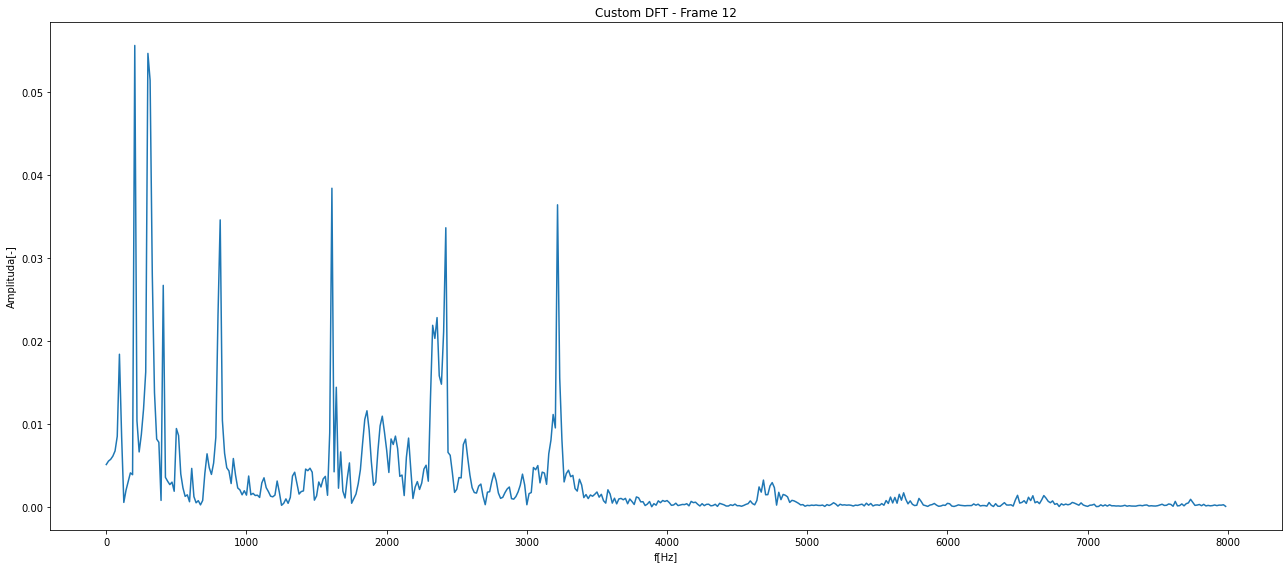
\includegraphics[scale=0.5,keepaspectratio]{Figure_5}
	\caption{Custom implementovaná funkce DFT}
\end{figure}
\end{landscape}

\begin{landscape}
\begin{figure}[H] 
	\centering
	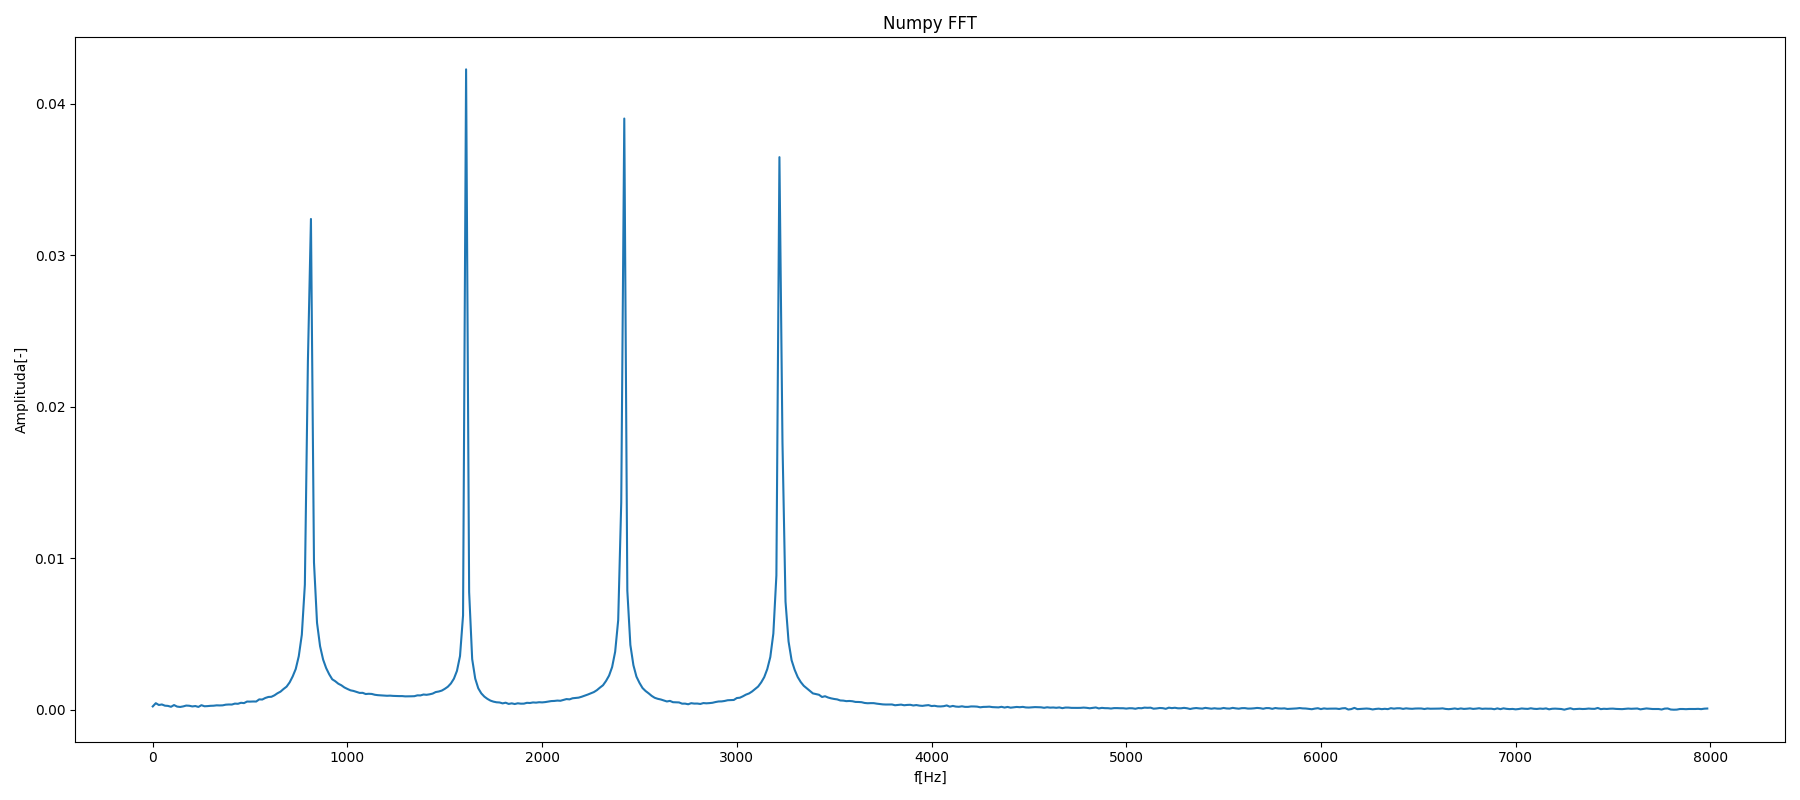
\includegraphics[scale=0.5,keepaspectratio]{Figure_4}
	\caption{Buildin FFT z knihovny numpy}
\end{figure}
\end{landscape}